% Waveforms: figures/paper/supplemental/s08_pulse_modifications.{pdf,npz}.
% Reproduce with scripts/make_supplemental_figures.py --only pulse_modifications.
% Midpoint comparison: outputs/sine_echo_transition_comparison/T{0,4,8,16}ns.npz
% and provenance.json; leakage is max(Pf_narrow), not maximum transient leakage.
% Matched linewidth/contrast: figures/paper/03_pulse_improvement_provenance.json
% and 03_pulse_improvement_metrics.csv; contrast uses dip_metrics, not SNR.
\section{Pulse Modifications: Phase Inversion, DRAG, and Cutoff-Edge Smoothing}
\label{sec:pulse-modifications}

The finite echo-root-Lorentzian pulse has two distinct sources of rapid waveform variation:
the midpoint sign reversal and the turn-on and turn-off at the cutoff.
We examine modifications of these features separately from the derivative
quadrature used for DRAG. This distinction matters because smoothing the
midpoint can suppress population transfer to $\lvert f\rangle$ without
removing the spectral effects of the outer edges, while DRAG alone need
not narrow the central spectroscopy dip. The separate effects are examined
with three-level simulations. The experimental comparison in
Fig.~\ref{fig:drag-beta-optimization}(d) tests a combined change of
midpoint smoothing and DRAG, rather than either modification in isolation.

Table~\ref{tab:pulse-modification-overview} summarizes the role of each
modification before the separate comparisons below.

\begin{table}[!ht]
    \caption{Pulse modifications and the limitations they address.
    The effects listed are established by the separate simulation
    comparisons below; the SNR is an ideal shot-noise estimate.}
    \label{tab:pulse-modification-overview}
    \renewcommand{\arraystretch}{1.15}
    \begin{ruledtabular}
    \begin{tabular}{p{0.27\columnwidth}p{0.64\columnwidth}}
    Modification & Problem and benefit \\
    \hline
    \raggedright Midpoint smoothing &
    Abrupt sign reversal causes leakage into $\lvert f\rangle$.
    A finite sine transition suppresses final-state leakage and gives
    a finite derivative for DRAG
    (Fig.~\ref{fig:midpoint-leakage}). \\
    \raggedright DRAG quadrature &
    Drive-induced phase error displaces the spectral center.
    Adding $Q\propto dI/dt$, with $\beta\simeq-0.5$ in our convention,
    reduces center motion; it does not by itself narrow the dip
    (Fig.~\ref{fig:drag-beta-optimization}). \\
    \raggedright Polynomial outer-edge smoothing &
    Hard truncation contributes to high-drive broadening and loss of
    visibility. Endpoint subtraction and the $p=5$ window reduce
    broadening, improve contrast and ideal SNR, and maintain these
    improvements over a wider drive range at fixed DRAG
    (Fig.~\ref{fig:edge-smoothing-results}). \\
    \end{tabular}
    \end{ruledtabular}
\end{table}

\subsection{The midpoint phase jump and its smooth implementation}

The ideal echo changes the carrier phase by $\pi$ at the pulse midpoint,
equivalently reversing the sign of its real envelope. In the numerical
implementation we replace the abrupt sign change by
\begin{equation}
    \begin{gathered}
    s_T(t)=
    \begin{cases}
        +1, & t<-T/2,\\
        -\sin(\pi t/T), & |t|\leq T/2,\\
        -1, & t>T/2,
    \end{cases}
    \\
    I(t)=\Omega_0 g(t)s_T(t),
    \end{gathered}
    \label{eq:pulse-modification-sign}
\end{equation}
where $g(t)$ is the unsigned, even envelope and $T$ is the transition
duration. The $T=0$ reference is an abrupt inversion. For $T>0$, both
$s_T$ and its first derivative are continuous. This interpolation passes
through zero in the real drive; it is not a constant-amplitude rotation
of the carrier phase. Its odd symmetry preserves zero signed pulse area.
Thus, for a real drive in the ideal resonant two-level model, the
cancellation argument of Sec.~\ref{sec:pulse-definition} still applies.
It does not imply exact cancellation in the dissipative three-level model
or after adding a noncommuting quadrature.

The saved transition-duration comparison isolates this change with
$L=20~\mu\mathrm{s}$, $c=0.005$, $\beta=0$, and no additional Stark-phase
correction. It uses $T_1=51.24~\mu\mathrm{s}$,
$T_2=7.31~\mu\mathrm{s}$, and
$\alpha/(2\pi)=-216~\mathrm{MHz}$. Figure~\ref{fig:midpoint-leakage}
shows the final $P_f$ over 201 detunings within $\pm0.5~\mathrm{MHz}$
at the highest drive, and its maximum over detuning for each of 25 drive
scales from 0 to $42.72~\mathrm{MHz}$. The largest final populations on
this grid are $3.19\times10^{-2}$, $7.23\times10^{-3}$,
$4.65\times10^{-4}$, and $2.55\times10^{-4}$ for $T=0$, 4, 8, and
$16~\mathrm{ns}$, respectively. Increasing $T$ from 0 to
$16~\mathrm{ns}$ therefore reduces the largest residual leakage by
about a factor of 125 on this grid.
This is final-state leakage, not the maximum transient occupation of
$\lvert f\rangle$. Halving the integration step from 0.5 to
$0.25~\mathrm{ns}$ at representative drive--detuning points changes
the final populations by at most $1.90\times10^{-5}$ across the four
transition durations. The subsequent matched waveform comparisons use
the same $16~\mathrm{ns}$ inversion with and without DRAG.

\begin{figure*}[!tp]
    \centering
    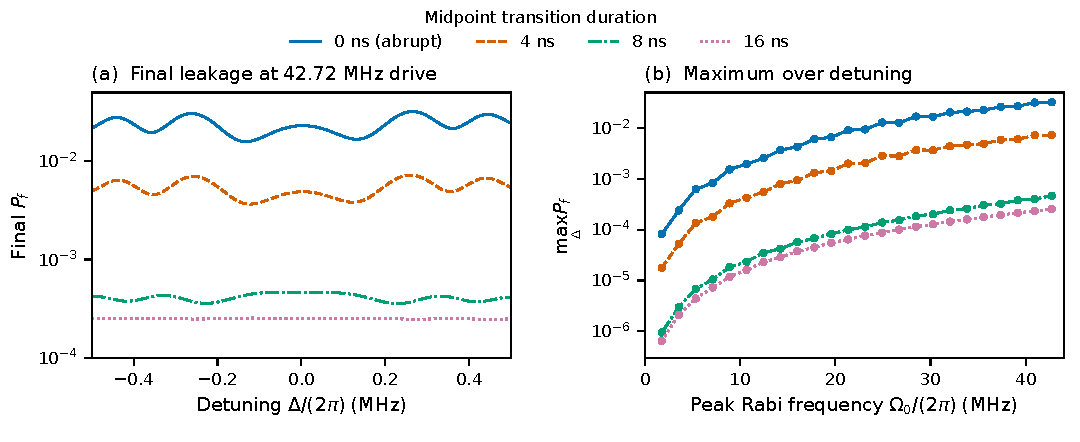
\includegraphics[width=\textwidth]{../figures/paper/supplemental/midpoint_smoothing_leakage.pdf}
    \caption{Simulated suppression of final-state leakage by smoothing
    the midpoint inversion of the echo-root-Lorentzian pulse.
    Curves compare $T=0$ (abrupt), 4, 8, and $16~\mathrm{ns}$ with
    $L=20~\mu\mathrm{s}$, $c=0.005$, and $\beta=0$ ($Q=0$).
    (a) Final $P_f$ versus detuning at
    $\Omega_0/(2\pi)=42.72~\mathrm{MHz}$.
    (b) Maximum final $P_f$ over the 201 sampled detunings within
    $\pm0.5~\mathrm{MHz}$, versus peak drive. Markers denote saved
    simulation amplitudes; lines connect samples without fitting or
    smoothing. Both leakage axes are logarithmic. The zero-drive point,
    for which $P_f=0$ in every case, is omitted from (b).
    The three-level model and convergence checks are specified in the text;
    the plotted population is evaluated after the pulse and is not the
    maximum transient occupation of $\lvert f\rangle$.}
    \label{fig:midpoint-leakage}
\end{figure*}

\subsection{DRAG acts on the complete signed waveform}

Using the complex-drive convention $I-iQ$, the DRAG quadrature
\cite{motzoi_drag_2009,gambetta_analytic_2011} is
\begin{equation}
    Q(t)=-\frac{\beta}{|\alpha|}\frac{dI}{dt}
    =-\frac{\beta\Omega_0}{|\alpha|}
    \left[g'(t)s_T(t)+g(t)s'_T(t)\right],
    \label{eq:pulse-modification-drag}
\end{equation}
where $\alpha$ is an angular frequency. Both the envelope derivative and
the derivative of the midpoint inversion are included. Applying DRAG
only to the unsigned envelope would omit the contribution where the
signed drive changes most rapidly. A finite $T$ regularizes that
contribution, whereas the derivative of an ideal instantaneous sign
change is singular.

The waveform and cutoff comparisons below use $\beta=-0.5$ in this
convention, motivated by the phase-compensation condition and numerical
scan that follow. No additional drive-phase correction is applied.

\subsection{Choice of the DRAG coefficient}

The value $\beta=-0.5$ has a perturbative phase-compensation motivation.
For a weakly anharmonic oscillator with the transmon matrix-element
ratio $\sqrt{2}$, the leading-order half-derivative DRAG solution removes
the phase error associated with the AC-Stark shift without an additional
time-dependent detuning control~\cite{gambetta_analytic_2011}. In the
quadrature convention used here, this gives
\begin{equation}
    Q_{\mathrm{phase}}(t)\simeq-\frac{1}{2\alpha}\frac{dI}{dt}
    =\frac{1}{2|\alpha|}\frac{dI}{dt},
    \qquad \beta_{\mathrm{phase}}=-\frac12.
    \label{eq:drag-half-derivative}
\end{equation}
This condition compensates the leading dynamical phase error; it does
not make the instantaneous dressed AC-Stark shift vanish. The central
minimum of a finite echo spectrum also depends on interference,
dissipation, and the cutoff, so its optimal coefficient need not be
exactly $-0.5$ or coincide with the minimum-leakage coefficient.

Figure~\ref{fig:drag-beta-optimization} tests this choice for the
$20~\mu\mathrm{s}$, $c=0.005$, $16~\mathrm{ns}$ sine-smoothed
echo-root-Lorentzian pulse, using the same three-level parameters as the
preceding leakage comparison. We scan 35 coefficients over
$-1\leq\beta\leq0$, with spacing 0.005 near $-0.5$, and hold all other
pulse parameters fixed. At seven equally spaced drive amplitudes from
10 to $42.72~\mathrm{MHz}$, the central minimum of $P_e$ is located
on a $[-60,60]~\mathrm{kHz}$ detuning grid with $1~\mathrm{kHz}$ spacing
and refined by a parabola through the minimum and its two neighbors.
The objective is the RMS center offset about zero detuning,
\begin{equation}
    J(\beta)=\left[\frac{1}{7}\sum_{j=1}^{7}
        \left(\frac{\Delta_{\min,j}(\beta)}{2\pi}\right)^2
        \right]^{1/2}.
    \label{eq:drag-beta-objective}
\end{equation}
The smallest sampled value is $J=0.099~\mathrm{kHz}$ at
$\beta=-0.495$, compared with $0.125~\mathrm{kHz}$ at $-0.5$ and
$7.64~\mathrm{kHz}$ at zero. Repeating the three coefficients
$-0.500$, $-0.495$, and $-0.490$ with a $0.25~\mathrm{ns}$ time step
and $0.5~\mathrm{kHz}$ detuning spacing preserves their ranking and
changes individual centers by less than $0.10~\mathrm{Hz}$.
Thus $-0.5$ is close to the numerical optimum for this center objective,
rather than an exact universal optimum.

The experimental comparison in Fig.~\ref{fig:drag-beta-optimization}(d)
compares two measured settings: $\beta=0$ with an
abrupt inversion and $\beta=-0.22$ with a $16~\mathrm{ns}$ inversion,
for $L=50~\mu\mathrm{s}$ and $c=0.00075$ on the second qubit.
The coefficients are quoted in the acquisition convention. Each run's
mean accepted center over the displayed 10--$60~\mathrm{MHz}$ range is
subtracted; the RMS variations are 6.78 and $2.64~\mathrm{kHz}$,
respectively. These measurements demonstrate improved center stability
for the combined pulse change. Because both the quadrature and midpoint
smoothing change, they neither isolate the effect of $\beta$ nor
establish an experimental optimum at $-0.5$.

\begin{figure*}[!tp]
    \centering
    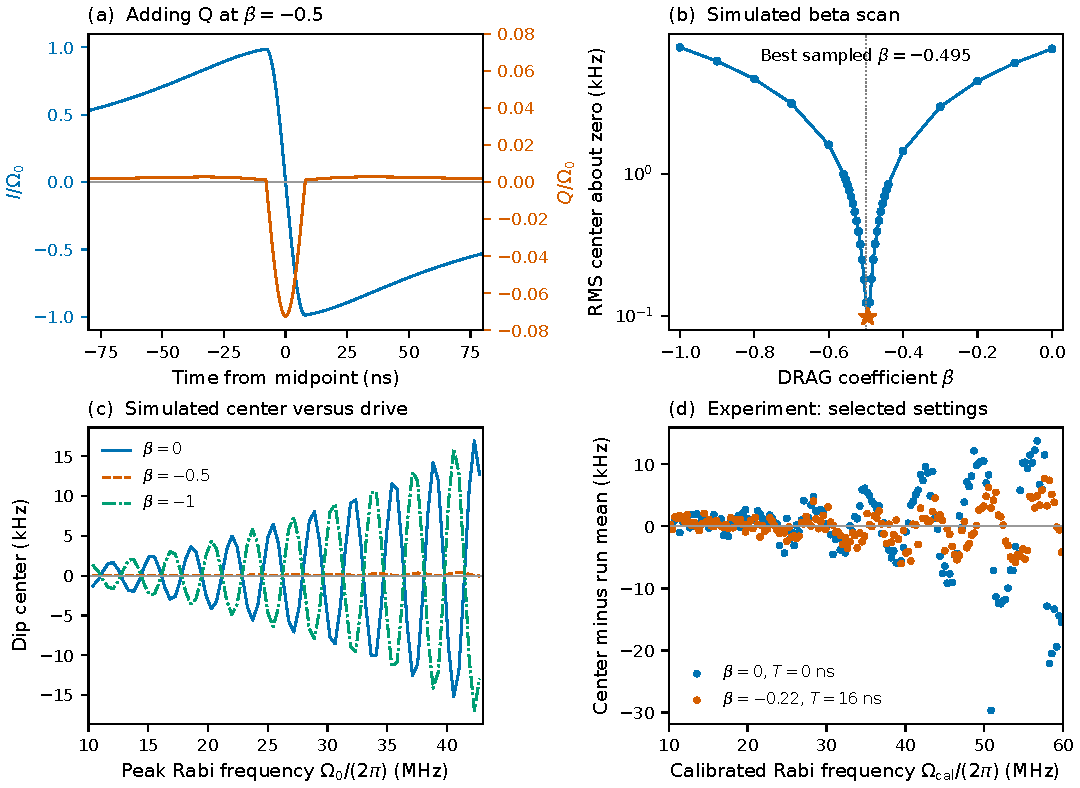
\includegraphics[width=\textwidth]{../figures/paper/supplemental/drag_beta_optimization.pdf}
    \caption{DRAG quadrature, simulated coefficient optimization, and
    experimental center stability. (a) Signed in-phase waveform (blue,
    left axis) and added quadrature (orange, right axis) at $\beta=-0.5$,
    with a $16~\mathrm{ns}$ inversion interval.
    (b) Simulated RMS center offset $J(\beta)$; the star marks the lowest
    sampled value at $-0.495$, and the dotted line marks $-0.5$.
    (c) Direct central minima of the saved simulated spectra for
    $\beta=0,-0.5,-1$; all three use identical midpoint smoothing.
    Panels (a)--(c) use $L=20~\mu\mathrm{s}$ and $c=0.005$ with no
    additional detuning correction. Lines connect sampled values.
    (d) Accepted Gaussian-fit centers from two measured $50~\mu\mathrm{s}$,
    $c=0.00075$ pulses, with one mean subtracted per run and no additional
    smoothing. Each acquisition used 2000 shots per point. The settings
    differ in both $\beta$ and inversion duration, as labeled; this panel
    is a measured comparison, not an experimental coefficient scan.}
    \label{fig:drag-beta-optimization}
\end{figure*}

\subsection{Smoothing the outer cutoff edges}

For the root-Lorentzian core,
\begin{equation}
    f(t)=\left[1+(t/\sigma)^2\right]^{-1/2},
    \qquad
    \sigma=\frac{L}{2}\frac{c}{\sqrt{1-c^2}},
\end{equation}
hard truncation at $t=\pm L/2$ leaves an amplitude jump of size $c$.
The polynomial correction first subtracts this endpoint value and then
multiplies by a symmetric window:
\begin{equation}
    g_p(t)=\frac{f(t)-c}{1-c}
    \left[1-\left(\frac{2t}{L}\right)^2\right]^p,
    \qquad |t|<L/2.
    \label{eq:pulse-modification-polynomial}
\end{equation}
It is zero outside the pulse. We use $p=5$, which makes the envelope
and its first five derivatives vanish at the boundaries. The corrected
envelope retains $g_p(0)=1$, is even, and uses the same
nominal scale $\Omega_0$. We apply neither pulse-area normalization nor
renormalization to the peak of the signed, smoothed waveform. The
cutoff $c$ consequently specifies the underlying core width, not the
nonzero endpoint amplitude of the corrected pulse. Figure~\ref{fig:pulse-modification-waveforms}
shows the envelope, turn-on edge, signed midpoint waveform, and DRAG
quadrature for
$L=30~\mu\mathrm{s}$ and $c=0.001$, corresponding to
$\sigma\simeq15~\mathrm{ns}$. Even with smoother outer edges, the sine
midpoint transition is only $C^1$ at its joins; outer-edge regularity
should not be confused with the regularity of the entire signed pulse.
The turn-off follows from the even symmetry of $g_p$. The signed
$I(t)$ is odd, whereas its derivative and hence $Q(t)$ are even.
The two contributions to $Q(t)$ in Eq.~\eqref{eq:pulse-modification-drag}
are shown separately: the midpoint term $g s_T^{\prime}$ produces the
central correction, while $g^{\prime}s_T$ also contributes away from the
inversion interval.

\begin{figure*}[!tp]
    \centering
    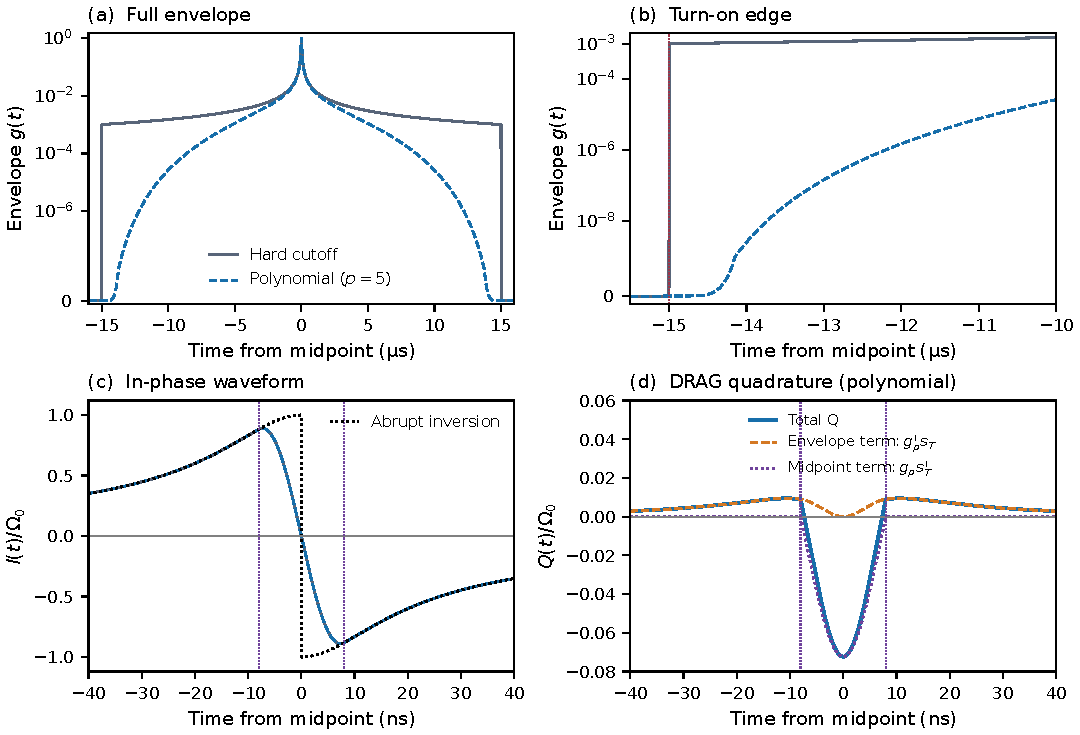
\includegraphics[width=\textwidth]{../figures/paper/supplemental/s08_pulse_modifications.pdf}
    \caption{Envelope shaping and DRAG for $L=30~\mu\mathrm{s}$,
    $c=0.001$, and a $16~\mathrm{ns}$ midpoint transition.
    (a) Unsigned hard-cutoff and polynomial-corrected ($p=5$) envelopes.
    (b) Turn-on edge; the turn-off is its mirror image. The envelope
    axes are logarithmic above $10^{-8}$ in (a) and $10^{-9}$ in (b),
    and linear below these values to include zero.
    (c) Signed in-phase waveform $I/\Omega_0$ near the midpoint,
    including the abrupt hard-cutoff inversion as a reference.
    (d) Polynomial-pulse DRAG quadrature $Q/\Omega_0$ for $\beta=-0.5$
    and $\alpha/(2\pi)=-216~\mathrm{MHz}$, decomposed into the
    envelope-derivative term $-\beta g_p^{\prime}s_T/|\alpha|$ and
    midpoint term $-\beta g_p s_T^{\prime}/|\alpha|$.
    Vertical dotted lines mark the $16~\mathrm{ns}$ inversion interval
    in (c),(d).
    The convention is $I-iQ$; $g(0)=1$ is held fixed without area or
    signed-peak renormalization.}
    \label{fig:pulse-modification-waveforms}
\end{figure*}

\subsection{Edge smoothing: linewidth, visibility, and drive robustness}

Figure~\ref{fig:edge-smoothing-results} isolates the outer-envelope
correction at fixed $\beta=-0.5$ and fixed $16~\mathrm{ns}$ midpoint
inversion. Both pulses use $L=30~\mu\mathrm{s}$, $c=0.001$, and the
same three-level coherence and anharmonicity parameters given above.
The only change is replacement of the hard-truncated envelope by
Eq.~\eqref{eq:pulse-modification-polynomial}, including both endpoint
subtraction and the $p=5$ window. The nominal peak scale is held fixed,
without area rematching. These are the saved matched simulations used
for the main-text pulse-improvement comparison, evaluated at 100 drive
scales from 0 to $100~\mathrm{MHz}$ and 201 detunings within
$\pm0.5~\mathrm{MHz}$.

The FWHM is extracted from the nearest half-depth crossings relative to
a linear background fitted over $0.4\leq|\Delta|/(2\pi)\leq0.5~\mathrm{MHz}$.
The contrast $C$ is the dip depth relative to this background, in
excitation-probability units. To quantify visibility at a fixed shot
budget, we additionally use the ideal SNR estimate from the saved
analysis. Let $p_c$ be the interpolated probability at the central dip
and $p_\pm$ the probabilities at detunings $\pm0.45~\mathrm{MHz}$.
For $N=1000$ independent binary measurements, with $N/2$ shots at the
center and $N/4$ at each shoulder,
\begin{equation}
    \begin{aligned}
    C_{\mathrm{sh}}&=\frac{p_++p_-}{2}-p_c,\\
    \sigma_C^2&=\frac{2p_c(1-p_c)+p_+(1-p_+)+p_-(1-p_-)}{N},\\
    \mathrm{SNR}_{\mathrm{ideal}}&=\frac{C_{\mathrm{sh}}}{\sigma_C}.
    \end{aligned}
    \label{eq:edge-ideal-snr}
\end{equation}
Here $C_{\mathrm{sh}}$ uses two fixed shoulders, whereas the plotted
$C$ uses the fitted background. This SNR assumes perfect classification
of $P_e$ and excludes assignment error, technical noise, drift, and the
measurement cost of locating the dip. It is a projection-noise estimate,
not a measured experimental SNR.

\begin{figure*}[!tp]
    \centering
    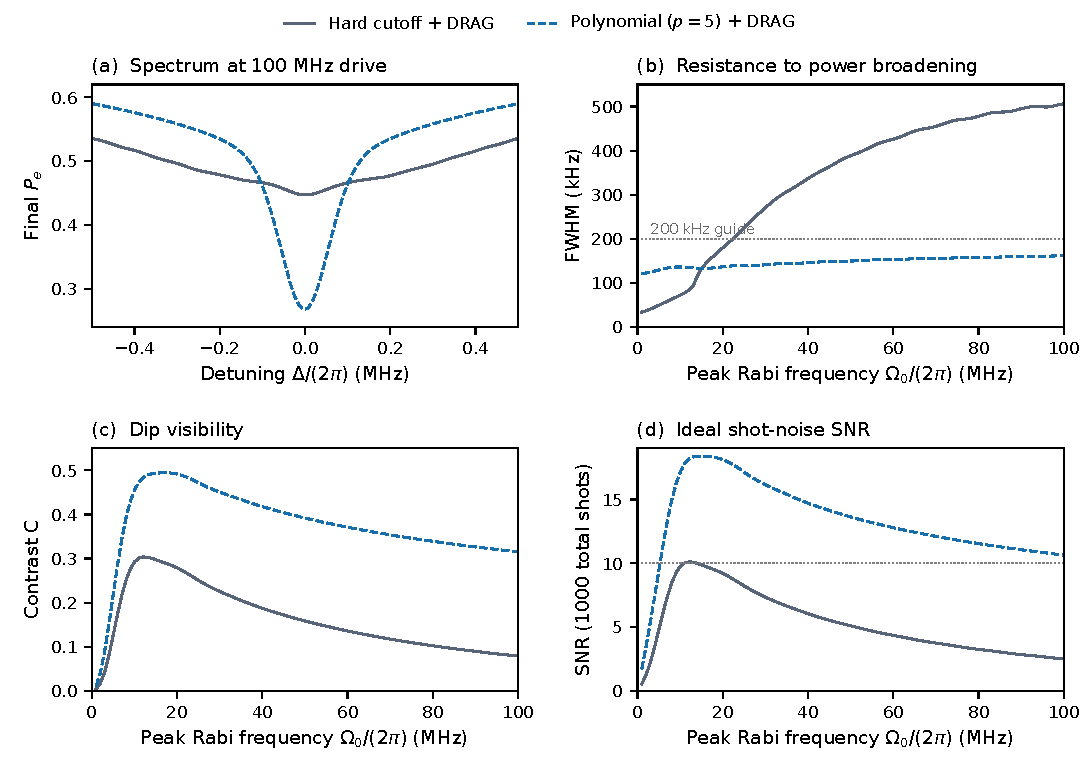
\includegraphics[width=\textwidth]{../figures/paper/supplemental/edge_smoothing_results.pdf}
    \caption{Effect of polynomial outer-edge smoothing at fixed DRAG.
    Gray solid curves show the hard cutoff; blue dashed curves add
    endpoint subtraction and the $p=5$ window. Both use
    $L=30~\mu\mathrm{s}$, $c=0.001$, $\beta=-0.5$, and a
    $16~\mathrm{ns}$ sine midpoint transition.
    (a) Simulated spectra at $\Omega_0/(2\pi)=100~\mathrm{MHz}$.
    (b) Dip FWHM, (c) background-referenced contrast $C$, and
    (d) ideal SNR from Eq.~\eqref{eq:edge-ideal-snr} versus peak drive.
    Dotted lines indicate illustrative criteria of FWHM $\leq200~\mathrm{kHz}$
    and SNR $\geq10$. All 50 sampled polynomial-pulse points in the
    50--$100~\mathrm{MHz}$ interval meet both criteria.
    Curves connect saved samples without
    additional smoothing or normalization; undefined zero-drive metrics
    are omitted.}
    \label{fig:edge-smoothing-results}
\end{figure*}

At $100~\mathrm{MHz}$, edge correction reduces the FWHM from 506.0 to
$161.8~\mathrm{kHz}$ and raises $C$ from 0.079 to 0.315. The ideal SNR
increases from 2.50 to 10.64. The improvement persists across all 50
sampled drive settings from 50.51 to $100~\mathrm{MHz}$: the corrected
pulse has worst-case FWHM $161.8~\mathrm{kHz}$ and minimum ideal SNR
10.64, compared with $506.0~\mathrm{kHz}$ and 2.50 for the hard cutoff.
Thus the polynomial correction maintains a narrower, more visible dip
throughout this high-drive interval. This is robustness to changing the
nominal drive scale; no stochastic amplitude-noise process is simulated.

The roles of the two corrections remain distinct. In the same saved
comparison, adding DRAG to the hard-cutoff pulse changes its
$100~\mathrm{MHz}$ FWHM from 484.8 to $506.0~\mathrm{kHz}$, so DRAG
alone does not produce the narrowing. The edge-corrected width also
remains above $1/(\pi T_2)=43.5~\mathrm{kHz}$. These results establish
an improvement for the specified pulse, drive interval, and readout
model, rather than a universal optimum or coherence-limited linewidth.
The final section examines the polynomial family's behavior over the
full cutoff and pulse-duration range.
